\documentclass[11pt]{report}

% Inconsolata untuk monospaced font

% \usepackage{fourier}
% \usepackage{venturis}
% \usepackage{cmbright}
\usepackage{inconsolata}  % can use [scaled=1.1]
\usepackage{graphicx}
\usepackage[english,bahasa]{babel}
\usepackage{makeidx}
\usepackage{a4wide}
\usepackage{fancybox}
\usepackage{hyperref}
\usepackage{wasysym}
\usepackage{url}
\usepackage[left=2cm,right=2cm,margin=2cm]{geometry}
\makeindex{}

\def\picscale{.37}
\setlength{\parindent}{0em}
\setlength{\parskip}{1em}
\linespread{1.2}

% Gambar ilustrasi
\newcommand{\fig}[1]{
  \begingroup
  \centering
  \includegraphics[scale=\picscale, bb=0 0 1366 718]{images/#1.jpeg}
  \label{fig:#1}
  \endgroup
}
\newcommand{\figL}[1]{
  \begingroup
  \centering
  \includegraphics[scale=\picscale, bb=0 0 1279 765]{images/#1.jpeg}
  \label{fig:#1}
  \endgroup
}
\newcommand{\figref}[1]{Gambar~\ref{fig:#1}}

% Tipe jendela Blender
\def\iconwnd#1{\includegraphics[height=10px,bb=0 0 36 25]{#1}}
\def\fontwnd#1{{\bfseries#1}}
\def\wnd3Dview{
  \iconwnd{icons/wnd3Dview.jpeg}~\fontwnd{3D View}}
\def\wndDopesheet{
  \iconwnd{icons/wndDopesheet.jpeg}~\fontwnd{Dopesheet}}
\def\wndFileBrowser{
  \iconwnd{icons/wndFileBrowser.jpeg}~\fontwnd{File Browser}}
\def\wndGraphEditor{
  \iconwnd{icons/wndGraphEditor.jpeg}~\fontwnd{Graph Editor}}
\def\wndOutliner{
  \iconwnd{icons/wndOutliner.jpeg}~\fontwnd{Outliner}}
\def\wndProperties{
  \iconwnd{icons/wndProperties.jpeg}~\fontwnd{Properties}}
\def\wndTimeline{
  \iconwnd{icons/wndTimeline.jpeg}~\fontwnd{Timeline}}
\def\wndUserPreferences{
  \iconwnd{icons/wndUserPreferences.jpeg}~\fontwnd{User Preferences}}
\def\wndUVImageEditor{
  \iconwnd{icons/wndUVImageEditor.jpeg}~\fontwnd{UV/Image Editor}}
\def\wndInfo{
  \iconwnd{icons/wndInfo.jpeg}~\fontwnd{Info}}
\def\modeObject{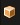
\includegraphics[height=10px,bb=0 0 20 25]{icons/modeObject.jpeg}~Object Mode}
\def\modeEdit{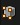
\includegraphics[height=10px,bb=0 0 20 25]{icons/modeEdit.jpeg}~Edit Mode}
\def\meshSelVertex{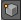
\includegraphics[height=10px,bb=0 0 25 25]{icons/meshSelVertex.jpeg}titik}
\def\meshSelEdge{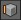
\includegraphics[height=10px,bb=0 0 25 25]{icons/meshSelEdge.jpeg}garis}
\def\meshSelFace{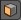
\includegraphics[height=10px,bb=0 0 25 25]{icons/meshSelFace.jpeg}bidang}

% Tombol
\def\key#1{\fbox{\bfseries\ttfamily#1}}
\def\ke{$\to$}
% \def\mki{
\includegraphics[height=10px,bb= 0 0 32 19]{icons/MKi.jpeg}}
% \def\mka{
\includegraphics[height=10px,bb= 0 0 32 19]{icons/MKa.jpeg}}
% \def\mtg{
\includegraphics[height=10px,bb= 0 0 32 19]{icons/MTg.jpeg}}
\def\mki{\fbox{MKi}}
\def\mka{\fbox{MKa}}
\def\mtg{\fbox{MTg}}

\title{{Workshop \textbf{Blender}}\\{\normalsize{}21-22 Mei 2011}}
\author{Adhi Hargo}
\date{}

\begin{document}

\maketitle{}


\chapter{Pemodelan + Penteksturan}

Bab ini memperkenalkan beberapa perangkat pemodelan dasar dalam Blender, dikemas sebagai tutorial untuk menciptakan gambar di bawah ini. Setiap langkah disertai ilustrasi, penjelasan ilustrasi dan file \texttt{.blend}. Semua tekstur disertakan dalam direktori \texttt{textures/}.

\fig{final}

\newpage{}

\fig{img-000}

Seperti inilah tampilan default Blender saat pertama kali dibuka. Untuk tutorial ini kita bisa memfokuskan perhatian pada jendela \textbf{1} dan \textbf{2} saja, tapi siapa tahu ada yang penasaran \smiley\ saya jelaskan sedikit fungsi masing-masing jendela dalam tampilan ini:

\begin{enumerate}
\item \wnd3Dview, tempat setiap objek 3D ditampilkan. Jendela paling penting, terutama saat pemodelan dan animasi. Tekan \key{Shift-F5} untuk mengubah tipe sembarang jendela menjadi \wnd3Dview.

\item \wndProperties\ di mana mayoritas pengaturan render, objek, material dan simulasi fisik dapat diakses.

\item \wndOutliner\ menampilkan daftar objek/data/pustaka yang terdapat dalam file \texttt{.blend}.

\item \wndTimeline\ menyediakan fasilitas marka dan navigasi waktu untuk keperluan animasi.

\item \wndInfo; fokus pada jendela ini pada menunya, yang memperlihatkan berbagai perintah, bantuan dan informasi penting terkait area kerja dan adegan yang tengah ditampilkan.
\end{enumerate}

Bila saat ini pertama kalinya Anda menggunakan Blender, sangat saya sarankan untuk `bermain-main' dengan antarmukanya. Membuat file baru (perintah \textbf{New} di menu \textbf{File} \wndInfo\ atau tekan \key{Ctrl-N}) akan mengembalikan Blender ke pengaturan semula.


\fig{peti-000}

\begin{enumerate}
\item Pertama, kita ubah terlebih dahulu unit ukur dalam Blender. Secara internal Blender memiliki unit ukur sendiri, biasa disebut Blender Unit. Tetapi ia dapat menampilkan bilangan dimensi dalam satuan riil yang lebih familiar, dalam contoh ini yaitu satuan metrik.

\item Blender memiliki fasilitas untuk membantu pemodelan yang relatif presisi, salah satunya adalah fasilitas \textsl{snap}. Jika saat memutar, menggeser atau mengubah skala benda, kita menahan tombol \key{Ctrl}, besar perubahan akan terkunci dalam unit tertentu. Di sisi kiri atas \wnd3Dview\ terlihat tulisan \textsf{10 Centimeters}, yang berarti unit snap dalam tampilan ini adalah setiap 10 sentimeter (tergantung grid paling kecil yang terlihat di layar).

  Dalam satuan metrik, ukuran kubus menjadi 2x2 meter.

\item Lihat di menu \wnd3Dview, terdapat dropdown yang memperlihatkan \modeObject. \modeObject\ berguna untuk manipulasi objek dalam ruang 3D, tapi untuk menyunting bentuk masing-masing objek, Blender harus berada dalam \modeEdit\ untuk objek tersebut. Masuk ke \modeEdit\ lewat dropdown ini, atau tekan \key{Tab}.

  Dari sini, dengan semua \meshSelVertex\ terpilih (tekan \key{A} bila belum), geser kubus 1 meter pada sumbu Z (\key{G}\ke\key{Z}\ke\key{1}).
\end{enumerate}

Dengan begini, titik pusat kubus berada di dasarnya. Kubus ini akan kita modelkan menjadi peti.


\section{Pemodelan}

\fig{peti-001}

\begin{enumerate}
\item Perangkat dasar pemodelan berbasis mesh pertama yang kita gunakan di sini adalah \textbf{Loop Cut and Slide} atau biasa hanya disebut \emph{loop cut}. Ia berguna untuk memotong serangkaian bidang (berapapun panjangnya). \emph{Loop cut} dapat diakses dari menu \textbf{Toolbox} \key{T}, atau dengan shortcut \key{Ctrl-R}.

\item Untuk memisahkan wujud kerangka dan badan peti, buat potongan-potongan seukuran lebar kerangka peti nantinya, yaitu 20cm. Cara termudah melakukannya adalah dengan terlebih dahulu menggeser posisi potong berhimpit dengan pinggir bidang, lalu dari pinggir menggeser masuk sejauh 20cm.
\end{enumerate}

\fig{peti-002}

Selanjutnya, kita bentuk tepi kerangka dan permukaan badan peti.

\begin{enumerate}
\item Perangkat yang kita pakai di sini adalah \textbf{Extrude Region}. Perintah ini berfungsi menambah \meshSelVertex,\meshSelEdge, atau \meshSelFace\ baru, tergantung apa komponen objek yang tengah dipilih. \emph{Extrude} dapat diakses dari menu \textbf{Toolbox}, atau dengan shortcut \key{E}.

\item Pilih satu-persatu \meshSelFace\ di tengah semua permukaan peti, ekstrusikan sejauh 10cm ke dalam.
\end{enumerate}

\fig{peti-003}

Sebelum masuk ke tahap penteksturan, kita atur dahulu pencahayaan. Belah dahulu jendela \wnd3Dview\ menjadi dua, buat salah satunya memperlihatkan perspektif kamera \key{Numpad 0}.

\begin{enumerate}
\item Tambahkan sebuah bidang planar sebagai lantai,
\item Buat duplikatnya \key{Shift-D},
\item Geser \key{G} dan putar \key{R} bidang duplikat tersebut agar menjadi dinding latar, dengan kedua bidang sedikit berpotongan.
\end{enumerate}

\fig{peti-004}

Selanjutnya, kita buat pengaturan awal cahaya.

\begin{enumerate}
\item Pertama, pilih objek lampu. Dalam tab \textbf{Data} \wndProperties, ubah jenis lampu menjadi \textbf{Sun}. Buat warnanya putih sedikit kekuningan, dan sesuaikan energi cahayanya sehingga menyerupai cahaya matahari saat siang.

\item Karena cahaya matahari bukan seperti satu lampu sorot raksasa di langit, kita perlu mengaktifkan opsi \textbf{Environment Lighting} dalam tab \textbf{World} \wndProperties. Ini membuat warna lingkungan turut mempengaruhi difusi cahaya. Pilih \textbf{Sky Color} sebagai sumber difusi cahaya sekunder, dan ubah warna \textbf{Horizon} menjadi putih kebiru-biruan.

  Ini membuat bagian objek yang tidak terkena cahaya matahari tidak sepenuhnya gelap, karena mendapat sedikit pembauran warna dari lingkungan sekitarnya.

\item Putar lampu matahari agar menyorot adegan secara menyerong. Berbeda dengan jenis lampu lain, posisi lampu berjenis \textbf{Sun} relatif terhadap objek lain tidak berpengaruh terhadap intensitas cahaya yang mengenai objek tersebut.

\item Naikkan kualitas bayangan dengan menambah nilai \textbf{Samples}-nya. Anda juga dapat mengatur nilai \textbf{Soft Size}, yang semakin besar nilainya, semakin memperhalus tepi bayangan.
\end{enumerate}

Bila kita render adegan ini, lewat menu \textbf{Render}\ke\textbf{Render Image} atau tombol \key{F12}, terlihat bahwa pengaturan cahaya di atas meniru efek pencahayaan siang hari.

\fig{peti-005}

Setelah bentuk mesh peti telah cukup terdefinisi, selanjutnya kita akan memberinya tekstur. Tekstur dalam Blender dapat dibagi ke dalam tiga tipe utama: tekstur \emph{gambar}, tekstur \emph{prosedural} dan tekstur \emph{berbasis nodus} untuk kombinasi kompleks kedua jenis tekstur sebelumnya. Untuk objek-objek dalam tutorial ini, kita akan gunakan tekstur gambar.

Teknik penteksturan berbasis gambar melibatkan pemetaan koordinat 3D dalam sumbu XYZ menjadi koordinat 2D dalam sumbu UV, prosedur yang umum dikenal sebagai \emph{UV mapping}. Proses ini dapat kita bayangkan seperti merobek dan memipihkan sebuah objek 3D menjadi bidang-bidang 2D. Meski proses tersebut berjalan otomatis, tapi kita tetap harus menentukan posisi ``robekan'' secara manual agar mendapat hasil yang rapi, agar memudahkan proses penteksturan.

\begin{enumerate}
\item Agar memudahkan penteksturan, buka jendela \wndUVImageEditor\ dan \wnd3Dview\ bersebelahan, atau ganti pengaturan tataletak jendela menjadi \texttt{UV Editing}.

\item Dalam \modeEdit, kita perlu menandai beberapa \meshSelEdge\ sebagai posisi ``robekan'' dengan perintah \textbf{Mark Seam} di menu \textbf{Toolbox} atau menu \textbf{Edge} \key{Ctrl-E}. Untuk menghapus tanda posisi robekan pada \meshSelEdge\ tertentu, tandai \meshSelEdge\ tersebut, lalu jalankan \textbf{Clear Seam}.

\item Posisi ``robekan'' diatur agar saat bangun peti ``dibongkar'' menjadi bidang planar, kita mendapat konfigurasi bidang yang mudah ditekstur. Setiap posisi robekan sudah ditandai, dalam ilustrasi di atas.

\item Bila objek siap dibongkar, pilih semua \meshSelEdge\ \key{A}, lalu jalankan \textbf{Unwrap}.

\item Konfigurasi bidang yang dihasilkan proses \emph{unwrap} biasanya perlu dirapikan sedikit, yang dalam ilustrasi ini hanya berupa mensejajarkan masing-masing \meshSelEdge.
\end{enumerate}

\fig{peti-006}

\begin{enumerate}
\item Agar dapat menyunting tekstur dengan editor eksternal, konfigurasi koordinat UV harus diekspor menjadi file lewat perintah \textbf{Export UV Layout} di menu \textbf{UVs} (saat objek berada pada \modeEdit).
\item Bila perintah tersebut belum muncul pada menu, add-on terkait harus diaktifkan terlebih dahulu dalam tab \textbf{Add-ons} jendela \wndUserPreferences, yang juga dapat diakses lewat shortcut \key{Ctrl-Alt-U} atau menu \textbf{File}\ke\textbf{User Preferences...} di jendela \wndInfo.
\item Aktifkan opsi \textbf{All UVs} agar tidak ada titik yang terlewat. Memilih format vektor SVG sebagai format ekspor, saya simpan file UV sebagai \texttt{peti.svg}.
\end{enumerate}


\section{Penteksturan}

\fig{gimp-001}

Penyunting gambar yang kita gunakan dalam tutorial ini adalah GIMP.

\begin{enumerate}
\item Bila format yang dipakai mengekspor tataletak UV adalah SVG, akan muncul dialog \textbf{Render SVG} saat kita membukanya dalam GIMP. Di sini kita dapat memutuskan untuk memakai resolusi gambar yang lebih besar, jika diperlukan.

  Dalam ilustrasi ini, saya menciptakan tekstur dengan resolusi lebih tinggi dibanding saat mengekspor SVG dari Blender (2048$\times$2048, dari sebelumnya 1024$\times$1024).
\item Ciptakan lapisan baru di bawah lapisan tataletak UV. Pada lapisan kedua inilah kita akan menciptakan tekstur objek, dengan lapisan hasil impor sebagai panduan.
\end{enumerate}

\fig{gimp-002}

Dalam tahap ini saya membahas dengan sedikit mendetail, salah satu cara menggabungkan beberapa file gambar atau tekstur yang sudah ada, untuk menciptakan tekstur baru yang sesuai dengan kebutuhan.

\begin{enumerate}
\item Perangkat GIMP pertama yang kita gunakan adalah \textbf{Fuzzy Select} \key{U}, untuk memilih satu wilayah pada gambar berdasarkan kedekatan warna. Dengan perangkat ini, klik \mki\ pada satu area gambar, dan seluruh area berdekatan dengan warna yang mirip akan terpilih. \textbf{Fuzzy Select} kita pakai untuk memberi tekstur pada badan peti.

  Saat lapisan tataletak UV \texttt{peti.svg} tengah aktif, tekan \key{Shift-\mki} pada setiap area UV badan peti. Dengan area seleksi tengah aktif, setiap kali kita membubuhkan tekstur, hanya area ini yang terpengaruh.

\item Perangkat GIMP yang kita pakai selanjutnya adalah \textbf{Clone} \key{C}. Perangkat ini menyampel area gambar dalam file dan lapisan tertentu, kemudian kita dapat membuat duplikatnya dalam file dan lapisan lain. Bila sumber dan tujuan \emph{clone} berbeda, kedua file harus tengah dibuka dalam GIMP.

\item Buka file gambar papan kayu \texttt{wooden\_floorboards\_021772.JPG}\footnote{Diambil dari \url{http://mayang.com/textures/} kategori \textbf{Wood}\ke\textbf{Manufactured}, disertakan dengan tulisan ini pada folder \texttt{textures/}.}, ubah ukuran gambar jika perlu disesuaikan lewat menu \textbf{Image}\ke\textbf{Scale Image}.

  Aktifkan perangkat \textbf{Clone} \key{C}. Tentukan gambar ini sebagai sumber \emph{clone} dengan menekan \key{Ctrl-\mki} di satu titik pada area gambar.  

\item Dalam file tekstur dengan lapisan gambar (bukan lapisan koordinat) terpilih, dan area seleksi aktif, tahan \mki\ dan sapukan kursor mouse ke setiap bidang persegi satu-persatu. Kita dapat memvariasikan tekstur papan pada masing-masing bidang dengan mengubah titik asal di sumber \emph{clone} \key{Ctrl-\mki}.

\item Setelah selesai, lapisan tataletak UV sebaiknya disembunyikan saja, agar memudahkan jika tekstur perlu direvisi.
\end{enumerate}

\fig{gimp-003}

\begin{enumerate}
\item Untuk tekstur kerangka, buat lapisan baru di bawah lapisan tekstur badan peti.

\item Buka file \texttt{wood\_texture\_9271241.JPG} dan \texttt{wood\_two\_knots\_9271240.JPG}\footnote{Diambil dari \url{http://mayang.com/textures/} kategori \textbf{Wood}\ke\textbf{Flat}, disertakan dengan tulisan ini pada folder \texttt{textures/}.}.

\item Dengan perangkat \textbf{Fuzzy Select} \key{U} atau \textbf{Rectangle Select} \key{R}, dan memanfaatkan tataletak UV di lapisan \texttt{peti.svg}, kita gunakan cara yang sama seperti saat mentekstur badan peti, pada tahap sebelumnya.

  Pilih area tertentu bersesuaian dengan lapisan UV (di lapisan tersebut, jika memakai \textsl{fuzzy select}, lalu buat \textsl{clone} gambar di lapisan tekstur kerangka peti. Gunakan kedua gambar --yang baru saja dibuka-- sebagai sumber \textsl{clone} secara bergantian, agar tekstur yang dihasilkan tidak terlalu monoton.

\item Kekurangan tataletak UV yang saya buat di sini adalah kurangnya robekan/\textsl{seam} sehingga ada bidang yang seharusnya persegi panjang terdistorsi menjadi trapesium (bidang kerangka peti yang bertemu dengan bidang badan peti). Ini akan mengakibatkan distorsi pada penampilan tekstur, misalnya garis-garis tegak lurus arah distorsi pada file tekstur akan terlihat melebar pada objek 3D.

  Kekurangan ini dapat kita akali dengan membuat alur kayu selalu sejajar arah distorsi, meski itu berarti harus memutar (\textbf{Rotate} \key{Shift-R}) salah satu file gambar\footnote{Rotasi hanya untuk keperluan \emph{cloning}, maka tidak perlu disimpan saat file ditutup.}. Dalam ilustrasi di atas, area seleksi aktif tengah saya \emph{clone} gambar yang telah dirotasi tersebut.

\item Setelah selesai, simpan file tekstur ini dalam format PNG, sebagai \texttt{peti.png}. Jangan lupa sembunyikan lapisan UV \texttt{peti.svg}.
\end{enumerate}

\section{Render}

\fig{peti-007}

Kembali ke Blender, kita pasang tekstur yang baru saja kita ciptakan dalam GIMP ke objek peti. Pertama, tekstur akan kita pasang agar setidaknya terlihat dalam \wnd3Dview.

\begin{enumerate}
\item Dalam jendela \wndUVImageEditor, buka file tekstur tersebut lewat menu \textbf{Image}\ke\textbf{Open Image} atau tombol \textbf{Alt-O}.

\item File tekstur \texttt{peti.png} termuat di \wndUVImageEditor.

\item Bila file tersebut dimuat di \wndUVImageEditor\ saat objek peti \underline{berada dalam \modeEdit}, kita dapat melihat wujud objek peti tersebut dengan tekstur terpasang, dengan mengubah mode tampilan \textbf{Textured} di jendela \wnd3Dview.
\end{enumerate}

Prosedur ini sudah cukup untuk melekatkan tekstur pada objek dalam viewport \wnd3Dview, tapi tekstur ini tetap belum ditampilkan saat adegan di-render.

\fig{peti-008}

Agar tekstur juga melekat pada objek dalam hasil render, tekstur tersebut harus dilekatkan terlebih dahulu pada sebuah material yang melekat pada objek tersebut. Semua jenis tekstur, termasuk tekstur gambar, tidak dapat dilekatkan langsung ke objek tanpa melalui material. Dalam Blender, sebuah objek dapat diberi banyak material, dan masing-masing material dapat diberi maksimal 18 tekstur.

\begin{enumerate}
\item Pertama, pastikan dalam tab \textbf{Material} jendela \wndProperties, bahwa peti ini telah memiliki setidaknya satu material (klik tombol \textbf{New} di bawah daftar material jika belum ada). 

  Dalam tab \textbf{Texture} \wndProperties, pastikan material tersebut telah memiliki setidaknya satu tekstur (klik tombol \textbf{New} di bawah daftar tekstur jika belum ada). Buat tipe tekstur ini \textbf{Image or Movie}.

\item Dari proses pemetaan UV sebelumnya, objek peti telah memiliki satu set koordinat UV. Agar tekstur gambar ini memanfaatkan sistem koordinat UV tersebut, pilih tipe koordinat \textbf{UV} dalam grup \textsf{Mapping}.

  Sebuah objek dapat memiliki beberapa set koordinat UV, maka tentukan nama spesifik set yang dipakai sebagai nilai \textbf{Layer}, terutama jika ada lebih dari satu set dalam objek.

\item Dalam grup \textsf{Image}, tentukan nama file tekstur yang digunakan. Bila prosedur menampilkan tekstur di viewport sebelumnya telah Anda lakukan, cukup tekan ikon gambar di kiri kotak teks dan pilih \texttt{peti.png}. Jika belum, buka lewat perintah \textbf{Open}.

\item Bila Anda render \key{F12} adegan ini, terlihat bahwa tekstur peti telah terpasang dengan objek dalam hasil render. Kualitas render masih dapat ditingkatkan sedikit dengan fitur \textbf{Ambient Occlusion}, yang menambah realisme dan kesan kedalaman dengan melemahkan cahaya lingkungan (\emph{ambient}) pada permukaan objek yang berdekatan dengan objek lain.

  Pencahayaan dalam adegan ini sudah cukup, dan mencampur AO dengan teknik \textbf{Add} akan membuatnya terlalu terang. Gunakan \textbf{Multiply} untuk sedikit meredupkan cahaya di area tertentu.
\end{enumerate}

\fig{peti-009}

\begin{enumerate}
\item Selanjutnya, kita pasang label pada peti tersebut. Caranya sama saja dengan sebelumnya, menggunakan pemetaan UV. Bedanya, kali ini seluruh bidang gambar dipetakan ke sebagian kecil bidang UV, kebalikan dari saat memasang tekstur keseluruhan objek.

  Peta koordinat UV yang dibutuhkan berbeda, maka kita buat baru di tab \textbf{Object Data} \wndProperties, dengan nama \texttt{decal}.

\item Dengan peta UV \texttt{decal} aktif, muat file \texttt{decal.png}\footnote{Disertakan dengan tulisan ini pada folder \texttt{textures/}.}. Dalam jendela \wnd3Dview\ dengan mode tampilan \textbf{Textured}, kita lihat tekstur label memenuhi seluruh permukaan peti. Ini karena gambar secara implisit dipetakan berulang terhadap peta UV. Sebenarnya tidak berpengaruh secara langsung terhadap tampilan objek saat render, namun dapat kita akali dengan memampatkan semua bidang UV yang tidak diperlukan menjadi satu:

  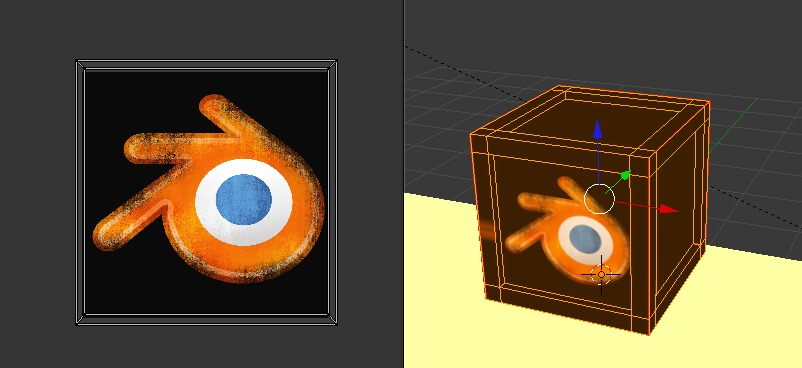
\includegraphics[scale=\picscale, bb= 0 0 802 368]{images/peti-009-s.jpeg}

  Caranya, pilih beberapa vertex, lalu ubah skala menjadi 0 (\key{S}\ke\key{0}).

\item Selanjutnya, pasang gambar label sebagai tekstur baru dengan memakai set koordinat UV \texttt{decal}, dalam grup \textsf{Mapping}. Dalam grup \textsf{Image}, aktifkan opsi \textbf{Premultiply} agar warna di balik tekstur bisa muncul (bila tidak, yang muncul warna putih sehingga transisi warna tekstur cenderung kasar).

\item Untuk perluasan gambar, pilih metode \textbf{Clip} agar gambar label tidak berulang, memenuhi seluruh permukaan peti.
\end{enumerate}

\fig{final}

Semua peti lain dalam adegan ini hanya duplikat-terkait dari objek peti yang baru kita buat. Duplikat-terkait/\textsl{linked duplicate}~\key{Alt-D} adalah duplikat objek dengan data objek yang sama; menyunting mesh satu objek akan turut mengubah semua duplikat terkait objek tersebut. Penteksturan lantai dan dinding menggunakan file \texttt{concrete\_020057.JPG} dan \texttt{uneven\_concrete\_wall\_9033094.JPG}\footnote{Diambil dari \url{http://mayang.com/textures/} kategori \textbf{Wall}, disertakan dengan tulisan ini pada folder \texttt{textures/}.}, dengan cara yang sama dengan mentekstur peti, meski lebih sederhana karena mesh-nya hanya terdiri atas satu \meshSelFace.

\chapter{Animasi + Render}

Bab ini memperkenalkan perangkat-perangkat animasi dasar dalam Blender, dirangkum sebagai tutorial animasi logo:

{\centering{}
\includegraphics[scale=\picscale, bb=0 0 960 540]{images/logo.jpeg}\\}

Animasi, terutama animasi CGI (``animasi 3D'') adalah bidang yang sepintas terlihat sederhana bagi orang awam, namun segera terasa kompleks dan tidak intuitif begitu sang awam ingin membuat gerakan, bahkan gerakan sederhana sekalipun. Maka, meski bab ini pun berwujud tutorial sebagaimana bab tentang pemodelan, terlebih dahulu saya coba jelaskan konsep paling mendasar animasi CGI dalam ilustrasi berikut:

\fig{anim-000}

\begin{enumerate}
\item Semua objek 3D (yang dapat dilihat lewat \wnd3Dview) memiliki tiga properti dasar: \emph{lokasi}, \emph{rotasi}, dan \emph{skala}. Semuanya dipecah menjadi properti per sumbu koordinat X, Y dan Z.

\item Nilai semua properti tersebut dapat berubah terhadap waktu. Misalnya, dalam gambar di atas lokasi kubus tengah berubah dari koordinat $(0, -8, 0)$ di frame 0, ke $(0, -3, 0)$ di frame 80, berakhir di $(0, 0, 0)$ pada frame 100. Posisi kubus pada ketiga frame tersebut adalah posisi utama (posisi yang ditentukan animator), dan frame-frame itu sendiri umum disebut frame kunci atau \emph{keyframe}\footnote{Pengertian \emph{keyframe} dalam sisi teknis animasi CGI berbeda dengan \emph{keyframe} dalam disiplin animasi secara umum. Kita harus membedakannya terutama saat mempelajari animasi karakter.}.

  Perubahan nilai sebuah properti dapat dilacak dan dimodifikasi melalui jendela \wndGraphEditor\ \key{Shift-F6}. Di sini terlihat posisi frame kunci (titik-titik kuning), perpindahan di antara masing-masing dua frame kunci (garis dengan warna sesuai kode warna properti, di kolom kiri).

\item Kita bisa saja berpindah antar-frame lewat jendela \wndGraphEditor, tapi terkadang navigasi lebih nyaman dilakukan lewat jendela \wndTimeline. Di sini terdapat banyak perangkat navigasi seperti untuk berpindah antar frame, antar frame kunci, dan memainkan animasi.

\item Semua objek 3D, termasuk yang tidak terlihat saat render, memiliki properti yang dapat dianimasikan.

\item Dalam Blender\footnote{Tidak termasuk Blender versi sebelum 2.5.} tidak hanya properti objek dalam ruang 3D yang dapat dianimasikan. Hampir semua properti dalam sebuah adegan dapat diubah frame-demi-frame, termasuk resolusi render!
\end{enumerate}


\section{Persiapan ``Skenario''}

Sebelum mulai menganimasikan adegan, saya jabarkan dulu gerakan yang akan dibuat. Dan kebetulan karena saya sudah terlebih dulu mencoba, jadi tahu pada frame-frame berapa \textsl{keyframe} akan diperlukan \smiley. Deskripsi singkatnya:

\begin{quotation}
  Closeup pada \textsl{asterisk}\footnote{\textsl{asterisk}: karakter bintang.} berputar sedikit kencang, yang berhenti saat sepertiga-\textsl{asterisk} bergerak mendekat. Tepat pada saat kedua objek menempel, kamera bergerak menjauh, memperlihatkan logo secara utuh.
\end{quotation}

Sederhana, kan? Ada tiga objek yang akan kita animasikan:

\begin{itemize}
\item\textbf{Asterisk} berwarna putih redup. Berputar pada frame \textbf{1}-\textbf{50}.
\item\textbf{Sepertiga-asterisk} berwarna merah. Mendekati \textsl{asterisk} sedikit lambat, menempel pada frame \textbf{50}.
\item\textbf{Kamera} tahan closeup, lalu bergerak mundur pada frame \textbf{50}-\textbf{100}.
\end{itemize}

\section{Animasi}

\subsection{Asterisk}

\fig{logo-000}

Kita mulai dari yang relatif sederhana dulu: memutar \textsl{asterisk}.

\begin{enumerate}
\item Kita ubah dahulu tataletak jendela, menggunakan konfigurasi \textbf{Animation}.

\item Pasang dua \textsl{keyframe}, masing-masing untuk nilai \textbf{Rotation} di frame \textbf{1} dan \textbf{50}.

\item Saat memasang \textsl{keyframe}, kita dapat berpindah antar-frame dengan memindahkan kursor pada jendela \wndDopesheet, \wndGraphEditor, atau \wndTimeline. Tapi memanipulasi letak \textsl{keyframe}, misalnya jika salah meletakkan \textsl{keyframe} dan ingin mengkoreksinya, paling mudah dilakukan di jendela \wndDopesheet: pilih salah satu \textsl{keyframe} dengan menekan \mka, lalu geser \key{G} ke frame yang diinginkan.

\item Posisi objek dalam kedua \textsl{keyframe} tidak berubah, terlihat dari bentuk kurva pada \wndGraphEditor\ yang datar. Kita akan mengubahnya dalam langkah berikutnya.
\end{enumerate}

\figL{logo-001}

\begin{enumerate}
\item Dalam \wndGraphEditor, pilih titik \textsl{keyframe} pada frame \textbf{50} untuk kurva rotasi sumbu Y. Geser ke atas sejauh 360 (\key{G}\ke\key{Y}\ke\key{``360''}). Perubahan pada kurva rotasi sumbu Y, yang bergeser dari 0 di frame \textbf{1} ke 360 di frame \textbf{50} akan membuat \textsl{asterisk} berputar tepat satu lingkaran penuh. Anda dapat mengubah nilai ini untuk mengubah kecepatan, tapi pastikan nilainya berkelipatan 60 agar posisinya mirip dengan kondisi awal.

\item Secara default, interpolasi antar \textsl{keyframe} bertipe \textbf{Bezier} yang membuat perputaran objek semakin cepat saat meninggalkan \textsl{keyframe} pertama, dan semakin lambat saat menuju \textsl{keyframe} kedua. Agar kecepatan perputaran \textsl{asterisk} konstan, kita perlu tipe interpolasi \textbf{Linear}. Ubah lewat menu \textbf{Key}\ke\textbf{Interpolation Mode}\ke\textbf{Linear}, atau \key{Shift-T}\ke\key{1}.

\item Bila kita putar animasi ini, akan terlihat \textsl{asterisk} berputar konstan sampai frame \textbf{50}, saat nantinya ia menempel dengan sepertiga-\textsl{asterisk}.
\end{enumerate}

\subsection{Kamera}

\figL{logo-002}

\begin{enumerate}
\item Pindah ke frame \textbf{1}, letakkan kamera hingga hanya menampilkan profil 3D objek \textsl{asterisk}. Pasang \textsl{keyframe} lokasi dan rotasi \key{I}\ke\textbf{LocRot}. Berbeda dengan objek \textsl{asterisk} yang hanya berubah rotasinya, kamera berubah nilai lokasi dan rotasinya. Bila Anda tidak memasang \textsl{keyframe} \textbf{LocRot}, perubahan rotasi objek tidak akan terekam bersamaan dengan perubahan lokasi.

  Anda bebas memilih sudut pandang yang akan digunakan.

\item Kita perlu agar kamera tetap berada dalam posisi ini sampai frame \textbf{50}. Ini bisa dilakukan dengan hanya memasang \textsl{keyframe} di frame \textbf{50}, tepat sebelum kamera berpindah posisi, tapi bila ini bagian dari gerakan yang lebih panjang, kita perlu \textsl{keyframe} awal dan akhir. Lebih mudah melakukannya di \wndDopesheet, dengan menduplikat \key{Shift-D} salah satu \textsl{keyframe} dan menggesernya.
\end{enumerate}

\figL{logo-003}

Gerakan kedua dan terakhir untuk kamera: pindah ke frame \textbf{100}, mundurkan kamera sampai seluruh logo terlihat, lalu pasang \textsl{keyframe} \textbf{LocRot}.


\subsection{Sepertiga-Asterisk}

\figL{logo-004}

\begin{enumerate}
\item Untuk objek sepertiga-\textsl{asterisk}, \textsl{keyframe} \textbf{Location} pertama pada frame \textbf{50} saat telah menempel dengan \textsl{asterisk}. \textsl{Keyframe} kedua adalah saat objek masih di luar bidang pandang kamera.

\item Lokasi \textsl{keyframe} awal menentukan kecepatan objek. Di sini saya tentukan posisi \textsl{keyframe} tersebut pada frame \textbf{35}.
\end{enumerate}

\section{Render}

\figL{logo-005}

\begin{enumerate}
\item Nilai teks pertama dalam grup \textsf{Output} adalah lokasi dan nama file. Nilai defaultnya biasanya adalah folder tempat file-file temporer, \texttt{/tmp/} dalam Linux. Di sini saya tentukan nilainya \texttt{//logo}. Awalan ``\texttt{//}'' dalam path Blender berarti lokasi yang sama dengan file \texttt{.blend}. Path ``\texttt{//logo}'' artinya file hasil render berada di lokasi yang sama dengan file \texttt{.blend}, dengan awalan nama \texttt{logo}. Blender biasanya menambahkan wilayah frame dan ekstensi berdasarkan format secara otomatis, kecuali jika opsi \textbf{File Extension} dinonaktifkan.

  Menu \textsl{dropdown} tepat di bawah lokasi output menentukan format hasil. Kita dapat memilih format video (MPEG, AVI, \ldots) atau gambar diam (PNG, JPEG, \ldots). Di sini kita pilih format video Xvid.

\item Set nilai \textsf{Resolution} menentukan ukuran gambar yang dihasilkan. Di sini saya tentukan ukuran gambar HD, namun kemudian di-skala \textbf{50\%}. Set nilai \textsf{Frame Range} menentukan panjang animasi. Nilai defaultnya biasanya adalah \textbf{250}, namun di sini kita tentukan \textbf{150} saja.

\item Setelah semua parameter render diatur, animasi dapat mulai dirender dengan menekan tombol \textbf{Animation} dalam grup \textsf{Render}, atau menekan \key{Ctrl-F12}.
\end{enumerate}

\end{document}

%%% Local Variables: 
%%% mode: latex
%%% TeX-master: t
%%% End: 
